\documentclass[tikz]{standalone}

\begin{document}
\begin{tikzpicture}[node distance=10cm]
    \node[] (pre) {
        \begin{tikzpicture}[y={(0.02cm,0.6cm)},x={(0.5cm,0cm)}, z={(-1cm, 0.5cm)}, scale=1]
            \draw[fill=gray!25] (0, 0, -2) -- (8.5, 0, -2) -- (8.5, 11, -2) -- (0, 11, -2) -- cycle;
            \draw[fill=gray!5, dashed] (0, 0, -1) -- (8.5, 0, -1) -- (8.5, 11, -1) -- (0, 11, -1) -- cycle;
            \draw[fill=gray!35] (0, 0,  0) -- (8.5, 0,  0) -- (8.5, 11,  0) -- (0, 11,  0) -- cycle;
        \end{tikzpicture}
    };

    \node[right of=pre] (post) {
        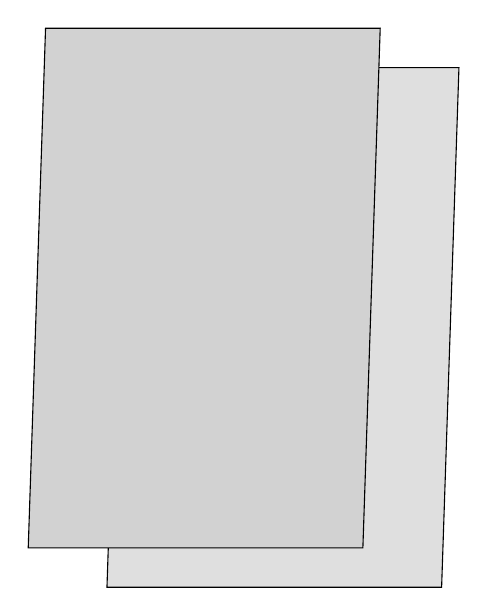
\begin{tikzpicture}[y={(0.02cm,0.6cm)},x={(0.5cm,0cm)}, z={(-1cm, 0.5cm)}, scale=1]
            \draw[fill=gray!25] (0, 0, -1) -- (8.5, 0, -1) -- (8.5, 11, -1) -- (0, 11, -1) -- cycle;
            \draw[fill=gray!35] (0, 0,  0) -- (8.5, 0,  0) -- (8.5, 11,  0) -- (0, 11,  0) -- cycle;
        \end{tikzpicture}
    };

    \draw[->, ultra thick] (pre) -- (post);

\end{tikzpicture}
\end{document}
